{\documentclass [10pt,a4paper]{book}
\usepackage{graphicx}

\begin{document}
\begin{flushright}
	
COLLABORATIVE E-RESEARCH      \textbf{79}
	
\end{flushright}
resides on a Windows server and provides a list of services, as illustrated in Figure 6.1. One of the unique features of the SharePoint service is the capacity for members of the team to alter the Web site directly from their Web browser, without having to craeate or upload docauments or HTML. pages. The communication services include threaded discussion groups that are presented in a format similar to typical newsgroups or computer conferences. Besides sharing documents, SharePoint provides customizable notification services using email to push notification to subseribers when information changes in either discussion groups or document libraries. 
SharePoint aslo has a polling feature that  allows members to query each other and instantly display the results. As seen in the screen capture in Figure 6.1, SharePoint is integrated with other Microsoft Office products, and thus will be most useful for teams that already use this suite of products. For example, SharePoint itself does not provide a  calendar feature, but can export items directly to the services built into Microsoft Outlook's calendar applications. SharePoint services must be installed on an internal company or institutional Web server and can  be purchased from external Web service providers. As the services and built into the cost of  the full-featured versions of Office XP, the cost for installation and operation is quite nominal; however, installation on a central server normally requires the cooperation of the information rechnology services of a central organization.
\begin{center}
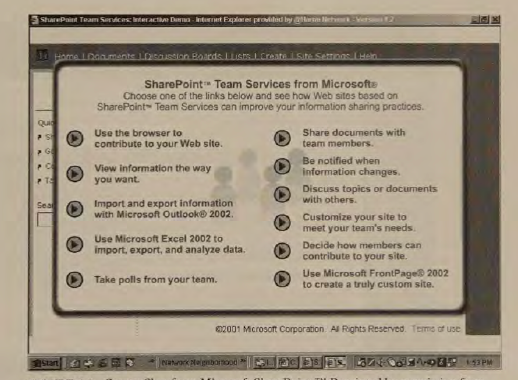
\includegraphics[scale=1]{1}
{FIGURE 6.1 Screen Shot from Microsoft SharePoint. ${}^{TM}$ Reprinted by permission from Microsoft Corporation.}
\end{center}
\end{document}
